\documentclass{article}
\usepackage[utf8]{inputenc}
\usepackage[polish]{babel}
\usepackage{ot1patch}   % ogonki do ą
\usepackage{enumitem}   % wyliczenia a b c d
\usepackage{graphicx}   % grafiki 
\usepackage{caption}    % tytuł wykresu
\usepackage[dvipsnames]{xcolor}
\usepackage{hyperref}   % linki
% marginesy
\addtolength{\textwidth}{4cm}
\addtolength{\hoffset}{-3cm}   
\addtolength{\textheight}{4cm}
\addtolength{\voffset}{-2,5cm}   % góra i dół strony

\title{Dokumentacja techniczna \\ \textbf{Wieloboki Voronoi}}
\author{Sylwia Marek \\ Ryszard Pręcikowski \\ \small{wtorek B, 14:40}}
\date{\today}

\begin{document}
\maketitle

\section{Wprowadzenie}
Projekt zawiera porównanie metod konstrukcji wieloboków Voronoi dla zadanego zbioru punktów na płaszczyźnie, za pomocą następujących algorytmów:
\subsection{Opis problemu}
Diagram Voronoi – podział płaszczyzny, który dla danego zbioru $n$ punktów generuje n obszarów, w taki sposób, że losowy punkt trafiający do danego obszaru znajduje się bliżej danego punktu (ze zbioru $n$ punktów), niż od pozostałych ($n-1$ punktów).
Do wyznaczania odległości została użyta metryka Euklidesowa.
\subsection{Algorytm Fortune'a}
Za pomocą algorytmu zamiatania tworzy diagram Voronoi dla zbioru punktów na płaszczyźnie.
\subsection{Algorytm Bowyera-Watsona (triangulacja Delaunay'a)}
Triangulacja Delaunay'a jest grafem dualnym diagramu Voronoi.
Na jej podstawie dla zadanej chmury punktów możliwe jest wyznaczenie diagramu Voronoi poprzez połączenie odcinkami środków okręgów opisanych na sąsiadujących trójkątach oraz utworzenie odpowiednich półprostych.


\section{Wymagane pakiety}
\subsection{Wizualizacja}
\begin{enumerate}
    \item numpy
    \item matplotlib
    \item json
\end{enumerate}

\subsection{Główne algorytmy}
\begin{enumerate}
    \item numpy
    \item matplotlib
    \item math
    \item random
    \item typing
    \item dataTypes
    \item computing 
    \item queue
    \item time
    
\end{enumerate}

\section{Źródła}
\begin{enumerate}
    \item M. de Berg, O. Cheong, M. van Kreveld, M. Overmars, \textit{Computational Geometry: Algorithms and Applications 3rd Edition}
    \item \url{https://en.wikipedia.org/wiki/Circumscribed_circle#Circumscribed_circles_of_triangles}

    \item \url{https://en.wikipedia.org/wiki/Delaunay_triangulation}

    \item \url{https://math.stackexchange.com/questions/213658/get-the-equation-of-a-circle-when-given-3-points?fbclid=IwAR2THXafz_TgKEfPpPuq4YnHrANNj17lxbkVWtMs0emioIWgW6_9q8Dzt4c}
    
    \item \url{http://www.multimedia.edu.pl/for_students/teaching_resources/biometry/files/cwiczenie6b.pdf}
    
    \item \url{https://pvigier.github.io/2018/11/18/fortune-algorithm-details.html}
    \item \url{https://stackoverflow.com/questions/85275/how-do-i-derive-a-voronoi-diagram-given-its-point-set-and-its-delaunay-triangula}
\end{enumerate}

\section{Opis programu/algorytmów}
Do wizualizacji algorytmów wykorzystano narzędzea do rysowania konstrukcji geometrycznych wykorzystywanych w trakcie laboratoriów. Jest ono napisane w języku Python3 i oparte o Projekt Jupyter. Wykorzystuje też biblioteki Numpy (który jest częścią biblioteki Scipy) oraz MatPlotLib.

\subsection{Algorytm Fortune'a}
\subsubsection{Struktury danych}
\begin{enumerate}
    \item Klasa Point 
    \newline
    \newline
    Klasa point reprezentuje punkt na płaszczyźnie dwuwymiarowej za pomocą współrzędnych x i y. Jednocześnie reprezentuje zdarzenia przechowywane w strukturze zdarzeń. Do tego celu potrzebne są pola:
    \begin{itemize}
        \item orderingY - reprezentujące współrzędną sortującą zdarzenia,
        \item arc – parabola, którą zaczyna dany punkt
        \item edge -krawędź wieloboku Voronoi najbliżej danego punktu.
    \end{itemize}
    Metody dostępne w tej klasie to:
    \begin{itemize}
        \item \_\_init\_\_- Metoda inicjalizująca punkt,
        \item setOrdering - Metoda ustawiająca współrzędną sortującą zdarzenia,
        \item toPQ - Metoda zwracająca krotkę używaną do przetrzymywania w strukturze zdarzeń,
        \item\_\_hash\_\_ - Metoda haszująca,
        \item \_\_eq\_\_ - Metoda sprawdzająca identyczność,
        \item \_\_repr\_\_ - Metoda zwracająca napis składający się z współrzędnych punktu.
    \end{itemize}
    
    \item Klasa HalfEdge 
    \newline
    \newline
    Klasa HalfEdge reprezentuje półprostą lub odcinek na płaszczyźnie. Zawiera dwa pola: start, end reprezentujące początek i koniec odcinka, jeśli jedno z tych pól jest puste to mamy do czynienia z półprostą. Dodatkowymi polami są next oraz prev, dzięki nim możliwe jest utworzenie podwójnie łączonej listy krwędzi.
    \newline
    Metody dostępne w tej klasie to:
    \begin{itemize}
        \item \_\_init\_\_- Metoda inicjalizująca (początek i koniec na tym etapie nie istnieją),
        \item\_\_hash\_\_ - Metoda haszująca,
        \item \_\_eq\_\_ - Metoda sprawdzająca identyczność,
        \item \_\_repr\_\_ - Metoda zwracająca napis składający się z punktu początkowego i końcowego.
    \end{itemize}
    
    \item Klasa RBNode 
    \newline
    \newline
    Klasa RBNode reprezentuje węzeł w drzewie czerwono – czarnym, jest elementem struktury stanu. Jest używana do przedstawienia paraboli. Zawiera pola potrzebne do funkcjonowania drzewa czerwono czarnego: ojciec, lewy, prawy syn oraz kolor (parent, left, right, color). Pola reprezentujące parabolę to:
    \begin{itemize}
        \item point – punkt, który inicjuje parabolę,
        \item leftHalfEdge, rightHalfEdge – półproste przecinające parabolę,
        \item prev, next – poprzednia oraz następna parabola,
        \item triggeredBy – zdarzenie kołowe, które było przyczyną powstania paraboli.

    \end{itemize}
    
    
    \item Struktura stanu 
    \newline
    \newline
    Struktura stanu reprezentowana jest przez drzewo czerwono czarne, w klasie RBTree.
    Klasa oferuje standardowe metody służące do używania drzewa czerwono czarnego, takie jak: sprawdzenie czy drzewo jest puste (isEmpty), ustawienie korzenia (createRoot), lewy obrót (left\_rotate), prawy obrót(right\_rotate), naprawę drzewa po dodaniu elementu (fix\_insert), zamianę węzłów miejscami (transplant), usunięcie węzła (delete), naprawę drzewa po usunięciu (delete\_fixup), znalezienie minimalnego węzła (minimum).
    \newline
    \newline
    Metody specyficzne da struktury stanu:
    \begin{itemize}
        \item getNodeAbove – metoda zwracająca parabolę nad danym punktem,
        \item insertBefore – metoda wstawiająca parabolę przed daną parabolą,
        \item insertAfter – metoda wstawiająca parabolę po danej paraboli,
        \item replace – metoda podmieniająca starą parabolę na nową (w tym samym miejscu w drzewie)

    \end{itemize}

    \item Struktura zdarzeń 
    \newline
    \newline
    Struktura zdarzeń reprezentowana jest przez kolejkę priorytetową. Priorytet zdarzenia (punktu) jest definiowany przez pole orderingY.
    
    \newline
    \newline
    \item Dodatkowe metody potrzebne do poprawnego działania algorytmu to:
    \begin{itemize}
        \item getIntersectionOfParabolas – zwracająca punkt przecięcia się paraboli powstałych z dwóch podanych punktów, na danej współrzędnej y,
        \item getConvergencePoint – zwracająca środek okręgu oraz dolny punkt okręgu powstałego z trzech podanych punktów

    \end{itemize}
    
    \item Klasa Voronoi 
    \newline
    \newline
    Klasa Voronoi przechowuje oraz wyznacza diagram Voronoi dla podanego zbioru punktów.
    \newline
    \newline
    Pola zawierające się w tej klasie to:
    \begin{itemize}
        \item points – zbiór punktów wejściowych,
        \item events – struktura zdarzeń,
        \item beachLine – struktura stanu,
        \item notValidEvents – zbiór przetrzymujący nieprawidłowe zdarzenia kołowe,
        \item vertices – zbiór punktów powstałego diagramu Voronoi,
        \item listEdges – lista krawędzi diagramu Voronoi,
        \item lowerLeft – lewy dolny punkt obramowania,
        \item upperRight – prawy górny punkt obramowania.

    \end{itemize}
    Główną metodą w tej klasie jest metoda „solve”, która po wywołaniu generuje diagram Voronoi.
    \newline
    \newline
    Główny podział metod to rozróżnienie na obsługujące zdarzenia kołowe oraz zdarzenia punktowe.
    Zdarzenia punktowe obsługiwane są przez metodę handleSiteEvent, wywołuje ona metody podrzędne:
    \begin{itemize}
        \item breakArc – metoda dzieląca daną parabolę na trzy na danej współrzędnej y,
        \item addCircleEvent – metoda dodająca zdarzenie kołowe powstałe z trzech parabol
        
    \end{itemize}
    Zdarzenia kołowe obsługuje metoda handleCircleEvent, korzysta ona z następujących metod:
    \begin{itemize}
        \item addCircleEvent (opisana wyżej)
        \item removeArc – usuwa daną parabolę z struktury stanu,
        \begin{itemize}
            \item addEdge – dodaje krawędź do listy krawędzi diagramu,
        \end{itemize}
    \end{itemize}
    
    Metody pomocnicze:
    \begin{itemize}
        \item findBounds – metoda znajdująca punkty obramowania,
        \item getIntersectionWithBox – metoda znajdująca punkt przecięcia półprostej z obramowaniem,
        \item endHalfEdges – metoda kończąca wszystkie półproste (kończy w punkcie przecięcia z obramowaniem).

    \end{itemize}
    
    \newline
    Wyniki działania algorytmu reprezentowane są w klasie Voronoi przez:
    
    \begin{itemize}
        \item pole vertices – zbiór wierzchołków diagramu,
        \item pole listEdges – lista krawędzi
    \end{itemize}
Dodatkowo, dla każdego punktu ze zbioru wejściowego pole edge wskazuje na krawędź wieloboku otaczającego dany punkt, następnie dzięki polom next oraz prev krawędzi mamy dostęp do podwójnie łączonej listy krawędzi danego wieloboku.

    
\end{enumerate}
\subsubsection{Wizualizacja}
Wizualizacja przeprowadzona za pomocą narzędzia Jupyter Notebook.

\begin{enumerate}
    \item Klasa Visualization zajmuje się zapisywaniem do scen poszczególnych etapów działania algorytmu. Zawiera pola i metody odpowiedzialne za rysowanie poszczególnych elementów diagramu. Dla użytkownika najważniejszym polem jest pole scenes, zawierające wszystkie sceny wizualizacji.
    \item Klasa VoronoiVisualization to klasa dziedzicząca z klasy Voronoi, nadpisuje część metod w celu dodania do nich funkcjonalności związanych z wizualizacją, nowa metoda to addVisualization dodająca obiekt klasy Visualization.
\end{enumerate}
Aby poprawnie przeprowadzić wizualizację należy:
\begin{enumerate}
    \item Zdefiniować zbiór obiektów klasy Point (set),
    \item Stworzyć nowy obiekt klasy VoronoiVisualization, należy przekazać do konstruktora zbiór punktów oraz ustawić flagę steps na wartość True,
    \item Stworzyć nowy obiekt klasy Visualization, do konstruktora przekazujemy wcześniej utworzony obiekt Voronoi,
     \item Do obiektu Voronoi dodajemy wizualizację za pomocą metody addVisualization,
     \item Wykonujemy metodę solve.
    \item Definiujemy nowy obiekt klasy Plot, w konstruktorze przypisujemy do scenes pole scenes obiektu Visualization.
     \item Na obiekcie plot wykonujemy metodę draw, z argumentem False.

\end{enumerate}

\subsubsection{Opis algorytmu}
Algorytm Fortune’a opiera się na algorytmie zamiatania, działa w czasie O(n log n), oraz używa O(n) pamięci. Został zaprezentowany przez Stevena Fortune‘a w 1986 roku.
Miotłą w algorytmie jest pozioma linia poruszająca się w kierunku pionowym, z góry na dół.
Struktura stanu nazywana jest linią brzegową. Składa się z łuków paraboli, z których każda jest wyznaczana przez konkretny punkt zbioru wejściowego.
Punkty powyżej miotły zostały dołączone już do diagramu Voronoi, natomiast punkty poniżej nie zostały jeszcze rozważone.

\subsection{Triangulacja Delaunay'a}
Do obliczenia triangulacji użyty został algorytm Bowyera Watsona, następnie na jej postawie wyznaczone wieloboki Voronoi.

\subsubsection{Reprezentacja}
Poszczególne trójkąty reprezentowane są jako lista, zawierająca wierzchołki trójkąta, oraz wskazanie na sąsiednie trójkąty ($None$, jeżeli sąsiada nie ma).

\subsubsection{Dostępne funkcje}

\begin{enumerate}
    \item Triangulacja
    \begin{itemize}
        \item generate\_points - generuje losową chmurę $n$ punktów z zadanego przedziału
        \item det - oblicza wyznacznik macierzy (pole równoległoboku rozpiętego na wektorach)
        \item point\_inside - sprawdza, czy punkt leży wewnątrz trójkąta, czy poza nim 
        \item equals - sprawdza, czy dane trójkąty są takie same
        \item is\_empty - sprawdza, czy dany trójkąt istnieje
        \item triangle\_center - zawraca środek ciężkości danego trójkąta
        \item unit\_vector - zwraca wektor jednostkowy (wersor), określający kierunek i zwrot wektora danego 2 punktami płaszczyzny
        \item first\_triangle - odnajduje pierwszy trójkąt aktualnej triangulacji
        \item has\_been\_visited - sprawdza, czy dany trójkąt był juz odwiedzony
        \item find\_triangle - odszukuje trójkąt zawierający dany punkt, zaczynając od pierwszego trójkąta triangulacji, idąc po kolejnych sąsiadach
        \item remove\_triangle - całkowicie usuwa dany trójkąt, usuwając go również z listy sąsiadów dla każdego swojego sąsiada
        \item point\_on\_line - zwraca odpowiedni indeks, w zależności od tego, na którym boku trójkąta leży dany punkt, bądź $None$ jeżeli leży poza nim
        \item legal - sprawdza, czy krawędź jest legalna, tj. czy dany punkt leży na zewnątrz okręgu opisanego na danym trójkącie 
        \item triangle\_vertices - sprawdza, czy dane 2 punkty są wierzchołkami trójkąta
        \item get\_ngh - zwraca sąsiada danego trójkąta względem krawędzi zadanej 2 punktami, $None$, jeśli takowego nie ma
        \item get\_third\_point - zwraca 3 punkt trójkąta, gdy dane są 2 pozostałe
        \item on\_edge - sprawdza czy punkt leży na odcinku (danym 2 punktami)
        \item legalize - zamienia krawędź nielegalną na legalną (lokalnie Delaunay'a)
        \item change\_ngh - zmienia odpowiedniego sąsiada danego trójkąta
        \item find\_ngh\_with\_point - zwraca sąsiada trójkąta, takiego, który zawiera dany punkt 
        \item insert\_point - wstawia kolejny punkt do triangulacji
        \item triangulate - dokonuje triangulacji zadanej chmury punktów (wraz z 3 dodatkowymi punktami, tworzącymi tzw. $supertrójkąt$)
        \item triangle\_out\_of\_scope - sprawdza, czy trójkąt jest poza zakresem współrzędnych; jeżeli jakikolwiek wierzchołek nie mieści się w zakresie, to cały trójkąt także
        \item get\_result\_triangles - usuwa z triangulacji trójkąty spoza zakresu, tj. zawierające punkty dodane sztucznie ($supertrójkąt$)
        \item \textbf{delaunay} - główna funkcja, dokonująca triangulacji zadanej chmury punktów płaszczyzny (poprzez dodanie $supertrójkąta$, triangulację zbioru z dodatkowymi punktami, usunięcie nadmiarowych trójkątów); zwraca trójkąty triangulacji
    \end{itemize}
    
    \item Diagram Voronoi
        \begin{itemize}
            \item center\_of\_circumcircle - zwraca środek okręgu opisanego na danym trójkącie
            \item triangles\_to\_lines - zwraca krawędzi danego trójkąta, na podstawie jego wierzchołków
            \item find\_edges\_without\_ngh - zwraca krawędzi danego trójkąta z podziałem na posiadające sasiadujący trójkąt oraz nieposiadające takowego
            \item middle\_point - zwraca punkt środkowy odcinka (zadanego jako 2 punkty do niego należące)
            \item line\_intersection - zwraca punkt przecięcia odcinków (zadanych jako 2 punkty do nich należące)
            \item frame\_cross - zwraca punkt przecięcia półprostej z ramką, daną skrajnymi punktami (lewy dolny i prawy górny róg)
            \item \textbf{voronoi\_diagram} - główna funkcja, dokonująca podziału płaszczyzny na wieloboki Voronoi dla zadanego zbioru punktów, za pomocą triangulacji Delaunay'a; zwraca wierzchołki oraz krawędzi diagramu Voronoi
        \end{itemize}
\end{enumerate}

\subsubsection{Wizualizacja}
W celu uzyskania wizualizacji algorytmów należy uruchomić funkcję \textbf{voronoi\_diagram} z parametrem $visualize$ ustawionym na wartość $True$; zwrócone zostaną sceny odpowiednio dla triangulacji, jak i podziału na wieloboki Voronoi, które pozwalają na prześledzenie algorytmów krok po kroku. 
\newline 
\newline 
Istnieje również możliwość zwizualizowania samego efektu działania algorytmu triangulacji bez kolejnych kroków. Aby to uzyskać należy uruchomić funkcję \textbf{delaunay} z parametrem $visualize$ ustawionym na wartość $False$, a na zwróconych przez nią trójkątach wywołać funkcję \textbf{triangles\_to\_lines}.
\newline 
\newline
Podobnie można zwizualizować podział na wieloboki poprzez wywołanie funkcji \textbf{voronoi\_diagram} z parametrem $visualize$ ustawionym na wartość $True$, a na podstawie zwróconych wierzchołków i krawędzi utworzyć wykres. 

\subsubsection{Opis algorytmu}
Algorytm Bowyer'a - Watsona pochodzi z roku 1981, polega na skonstruowaniu powłoki pokrywającej punkty chmury poprzez dodanie 3 punktów pomocniczych tworząc trójkąt, który zawiera w swoim wnętrzu wszystkie punkty chmury. Jest to początkowa triangulacja. Następnie dokłada się kolejne punkty (w kolejności losowej), odnajdując trójkąt triangulacji, który go zawiera. W zależności od tego, czy punkt leży wewnątrz, czy na krawędzi trójkąta, odpowiednio dzieli się trójkąty, następnie następuje legalizacja krawędzi w nowo-powstałych trójkątach. Finalnie otrzymana triangulacja nie zawiera dodanych na początku 3 punktów. 
\newline
Korzystając z faktu, że triangulacja Delaunay'a jest grafem dualnym diagramu Voronoi, w stosunkowo łatwy sposób da się otrzymać podział płaszczyzny na wieloboki, poprzez połączenie środków okręgów opisanych na sąsiadujących ze sobą (uprzednio wyznaczonych) trójkątach. Jeżeli natomiast dany trójkąt nie ma sąsiada względem którejś z krawędzi, utworzona zostaje półprosta  o początku w środku okręgu, której przedłużenie jest symetralną boku boku trójkąta, względem którego nie ma sąsiada.

\section{Przeprowadzone testy}
Algorytmy działają poprawnie dla zbiorów danych większych od trzech punktów, jednocześnie nieposiadających punktów mających te same współrzędne x lub y.
\newline
Testy wydajnościowe zostały przeprowadzone na losowych zestawach danych, dla każdej ilości punktów zostały powtórzone osiem razy, aby uniknąć wpływu skrajnych przypadków na czas działania. Uśrednione wyniki zostały przedstawione graficznie na Rysunku 1.
\newline
\newline

\begin{minipackage}{\linewidth}
            \centering
            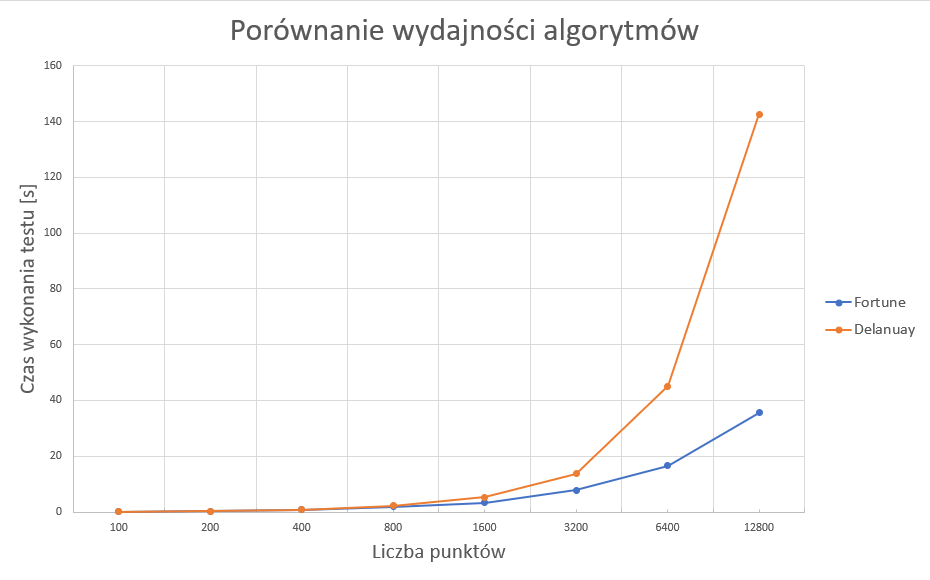
\includegraphics[width = 16cm]{testy.png}
            \captionof{figure}{Porównanie czasów działania obu użytych algorytmów}
        \end{minipackage}
        

\section{Przykładowe wyniki działania}
\subsection{Algorytm Fortune'a}
        \begin{minipackage}{\linewidth}
            \centering
            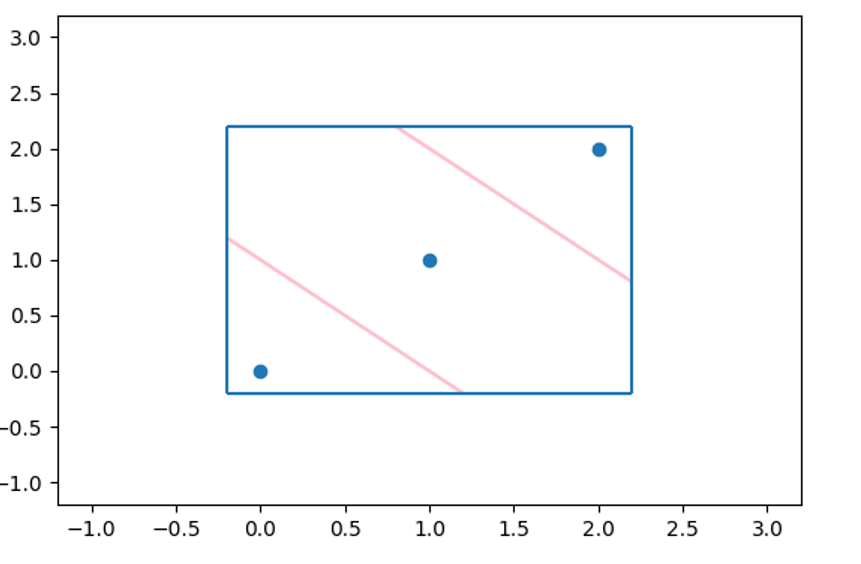
\includegraphics[width = 16cm]{fortuna_3.png}
            \captionof{figure}{Zestaw 3 punktów leżących na prostej}
        \end{minipackage}
        \begin{minipackage}{\linewidth}
            \centering
            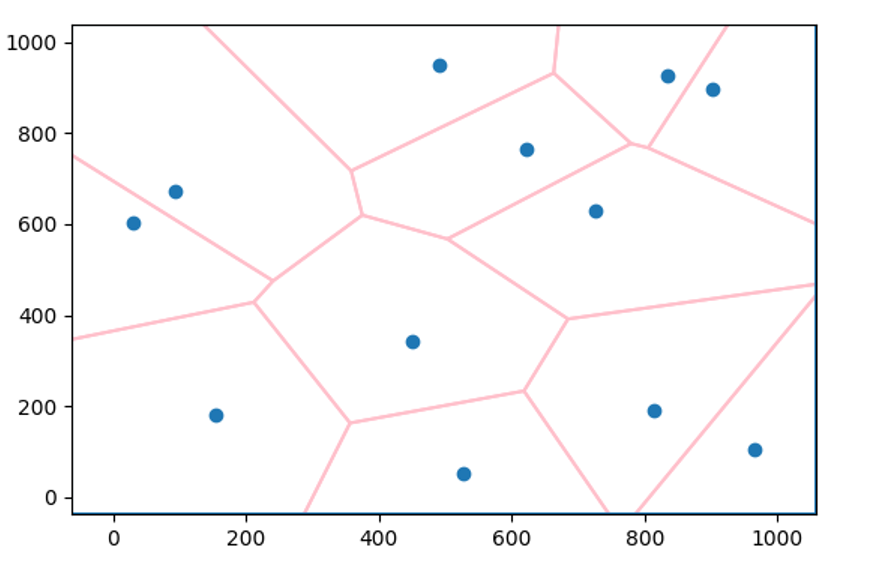
\includegraphics[width = 16cm]{fortuna_8.png}
            \captionof{figure}{Zestaw 8 losowych punktów}
        \end{minipackage}
        \begin{minipackage}{\linewidth}
            \centering
            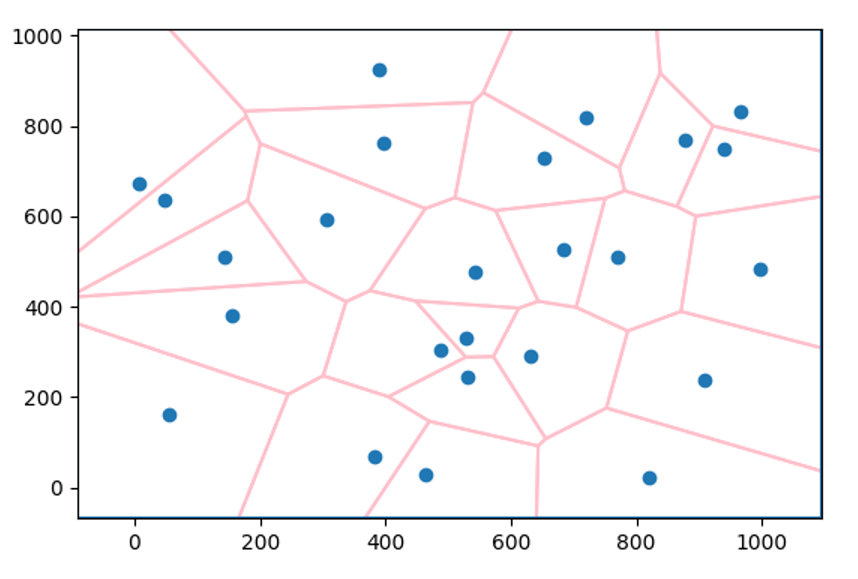
\includegraphics[width = 16cm]{fortuna_25.png}
            \captionof{figure}{Zestaw 25 losowych punktów}
        \end{minipackage}
        \begin{minipackage}{\linewidth}
            \centering
            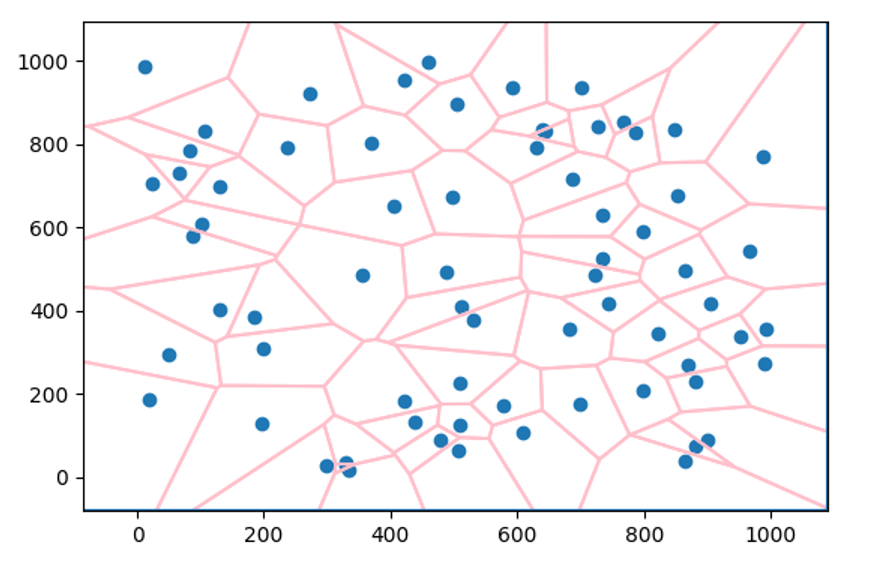
\includegraphics[width = 16cm]{fortuna_70.png}
            \captionof{figure}{Zestaw 70 losowych punktów}
        \end{minipackage}

\subsection{Algorytm na podstawie triangulacji Delaunay'a}
        \begin{minipackage}{\linewidth}
            \centering
            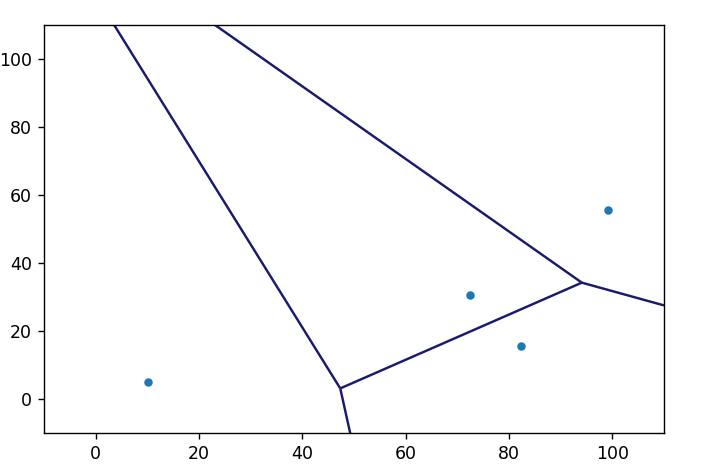
\includegraphics[width = 16cm]{del_4.png}
            \captionof{figure}{Zestaw 4 losowych punktów}
        \end{minipackage}
        \begin{minipackage}{\linewidth}
            \centering
            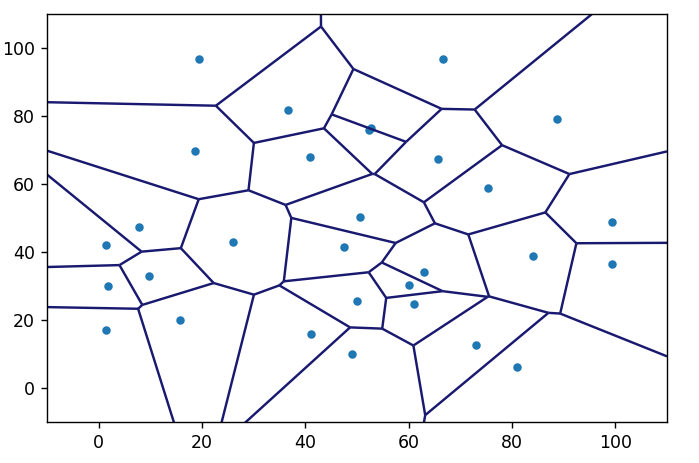
\includegraphics[width = 16cm]{del_30.png}
            \captionof{figure}{Zestaw 30 losowych punktów}
        \end{minipackage}
        \begin{minipackage}{\linewidth}
            \centering
            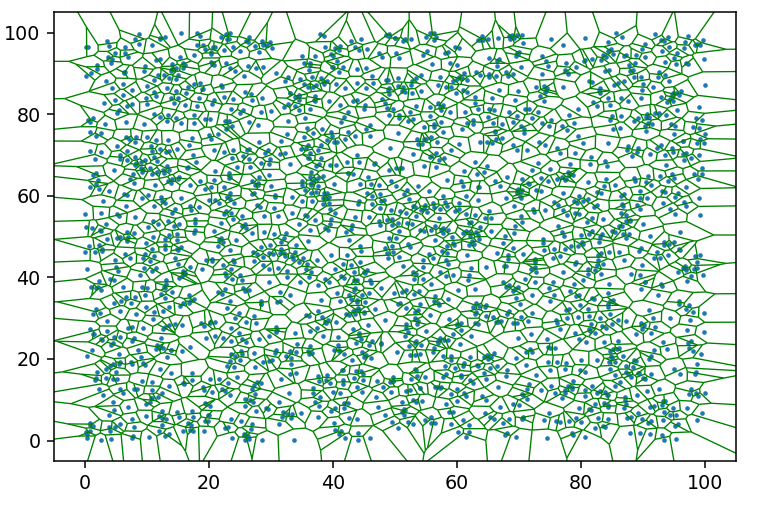
\includegraphics[width = 16cm]{del_2000.png}
            \captionof{figure}{Zestaw 2000 losowych punktów}
        \end{minipackage}
        
\subsection{Oba algorytmy na tym samym losowym zestawie danych}
\begin{minipackage}{\linewidth}
            \centering
            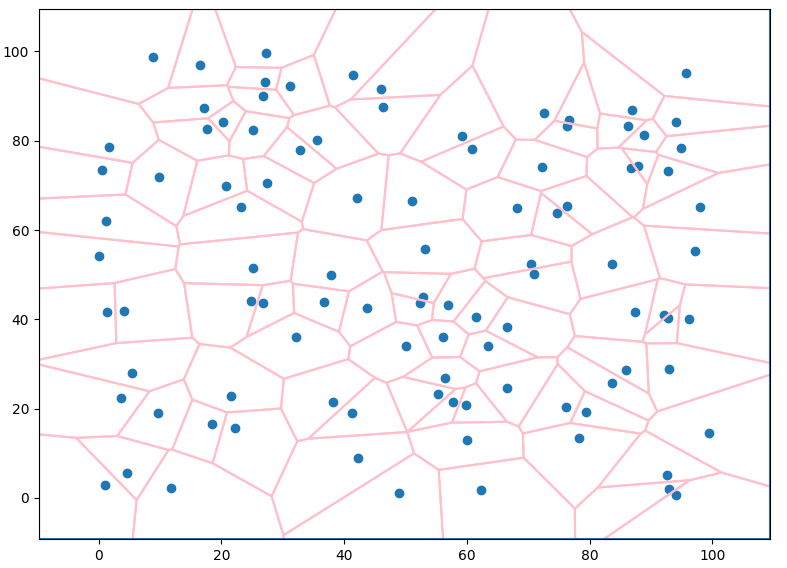
\includegraphics[width = 15cm]{100_fortuna.png}
            \captionof{figure}{Zestaw 100 losowych punktów - algorytm Fortune'a}
        \end{minipackage}
        \begin{minipackage}{\linewidth}
            \centering
            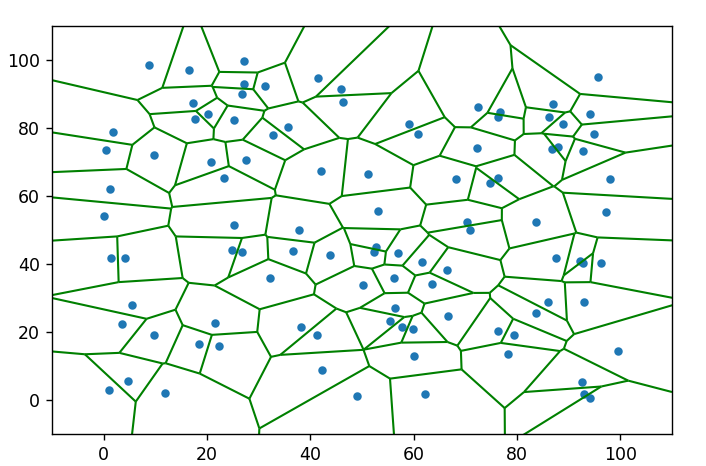
\includegraphics[width = 15cm]{100_del.png}
            \captionof{figure}{Zestaw 100 losowych punktów - algorytm na podstawie triangulacji Delaunay'a}
        \end{minipackage}
        
\section{Wnioski}
Oba testowane algorytmy wyznaczają wieloboki Voronoi dla zadanych punktów poprawnie, pod warunkiem, że zbiory są większe od 3 punktów oraz nie leżą one na tej samej prostej. Zgodnie z przewidywaniami algorytm Fortune'a wykazuje czasową przewagę nad algorytmem na podstawie triangulacji Delaunay'a (metoda Bowyer'a Watsona).

\end{document}
